\section{Prompt wording and question-paraphrase robustness}
\label{app:prompt-text}

All prompt families append the same answer format, ``\texttt{The answer is <short answer>},'' to the original or paraphrased question. They differ only in whether they add no cue (\texttt{B\_direct}), internal step-by-step reasoning (\texttt{C\_step\_only}), visual evidence (\texttt{D\_visual\_only}), or both reasoning and visual evidence (\texttt{A\_step\_visual}). Some main analyses use only the \texttt{B\_direct} and \texttt{D\_visual\_only} subset, while this diagnostic uses all four families.

The wording and question-paraphrase grid tests whether the evidence-to-answer effect is merely driven by wording. These analyses predate the final same-object sparse comparison and are retained as auxiliary identity and hidden-state diagnostics. The unified \modelgemma{} and \modelqwen{} analysis separates fixed-node strength from route-identity stability. Table~\ref{tab:wording-grid} summarizes the diagnostic counts and model-appropriate stability statistics. For Gemma, the two counts are fixed-node rows and target-aligned rows; for Qwen, they are candidate-metric rows and top-$K$ overlap rows; for LLaVA, they are evaluated condition keys and image--question samples. Node or feature overlap compares sparse identities, structural overlap compares Gemma graph edges or Qwen layer--position--feature identities, and the hidden positive fraction is the proportion of LLaVA condition keys with a positive hidden-restoration logit effect. NA denotes an unavailable quantity, not a zero effect. Route identity is only moderately stable, so these diagnostics do not establish fixed-node invariance or positive causal coverage by the fitted sparse tools.

\begin{table}[htbp]
\centering
\small
\caption{\textbf{Wording diagnostic matrix.} Counts use the row-specific units defined in the preceding text. Sparse-overlap columns apply to Gemma and Qwen; the hidden positive fraction applies to LLaVA.}
\label{tab:wording-grid}
\begin{tabular*}{\linewidth}{@{\extracolsep{\fill}}lrrrrr@{}}
\toprule
Analysis & \shortstack{Full\\count} & \shortstack{Analysis\\count} & \shortstack{Node/feature\\overlap} & \shortstack{Structural\\overlap} & \shortstack{Hidden positive\\fraction} \\
\midrule
Gemma graph & 524 & 414 & 0.280 & 0.183 & NA \\
Qwen route rediscovery & 4608 & 576 & 0.596 & 0.409 & NA \\
LLaVA hidden grid & 576 & 12 & NA & NA & 0.852 \\
\bottomrule
\end{tabular*}
\end{table}

Changing the question wording or prompt family can therefore change \emph{which sparse identities or hidden-effect pattern is observed}, even when the image evidence and answer remain the same. This observation establishes measurement sensitivity to wording; it does not by itself identify a different native computation. We therefore avoid claiming fixed-node invariance across prompts.

The LLaVA wording grid provides a hidden-level robustness check rather than a grouped-route identity test. Its hidden-logit positive fraction is $0.852$ overall and ranges from $0.833$ to $0.891$ across the reported prompt-family and question-variant summaries. Wording changes therefore modulate effect size without removing the hidden-level intervention signal.

\begin{figure}[htbp]
    \centering
    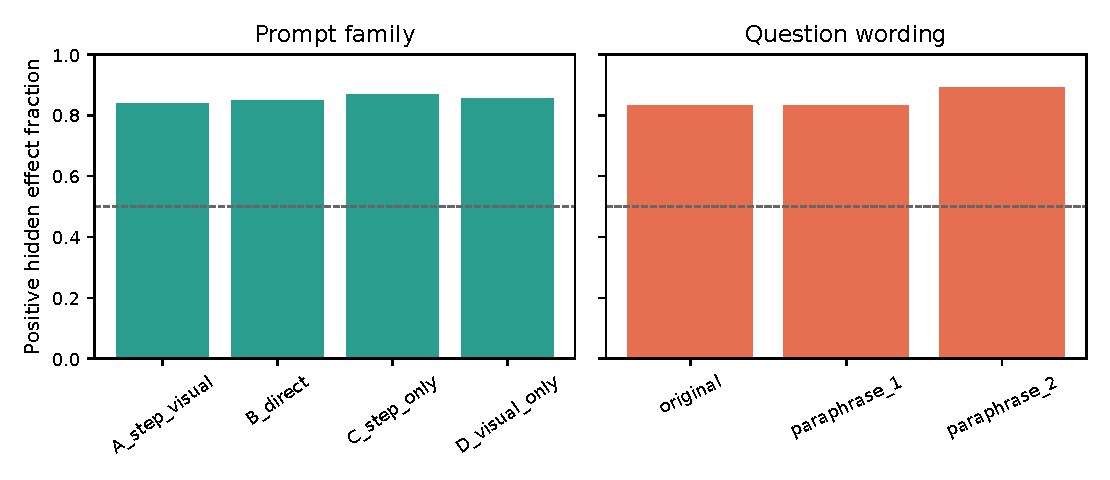
\includegraphics[width=0.88\linewidth]{figures/llava_prompt_text_grid.pdf}
    \caption{\textbf{LLaVA prompt and question-variant grid.} Cells summarize hidden-level effect direction across prompt families and paraphrases.}
    \label{fig:prompt-grid}
\end{figure}

Together, these diagnostics support a careful secondary conclusion: prompt and wording changes modulate observable sparse identity and hidden-effect allocation, but do not explain away the hidden-state evidence-to-answer dependence measured by the final intervention tests.

\FloatBarrier
